\section{Data and methods}
\label{sec:datamethods}

\subsection{Data}
\label{subsec:data}
%TODO mention data acquisition in each section
%TODO no table cause you reference each dataset

	\begin{figure}[ht]
		\centering
		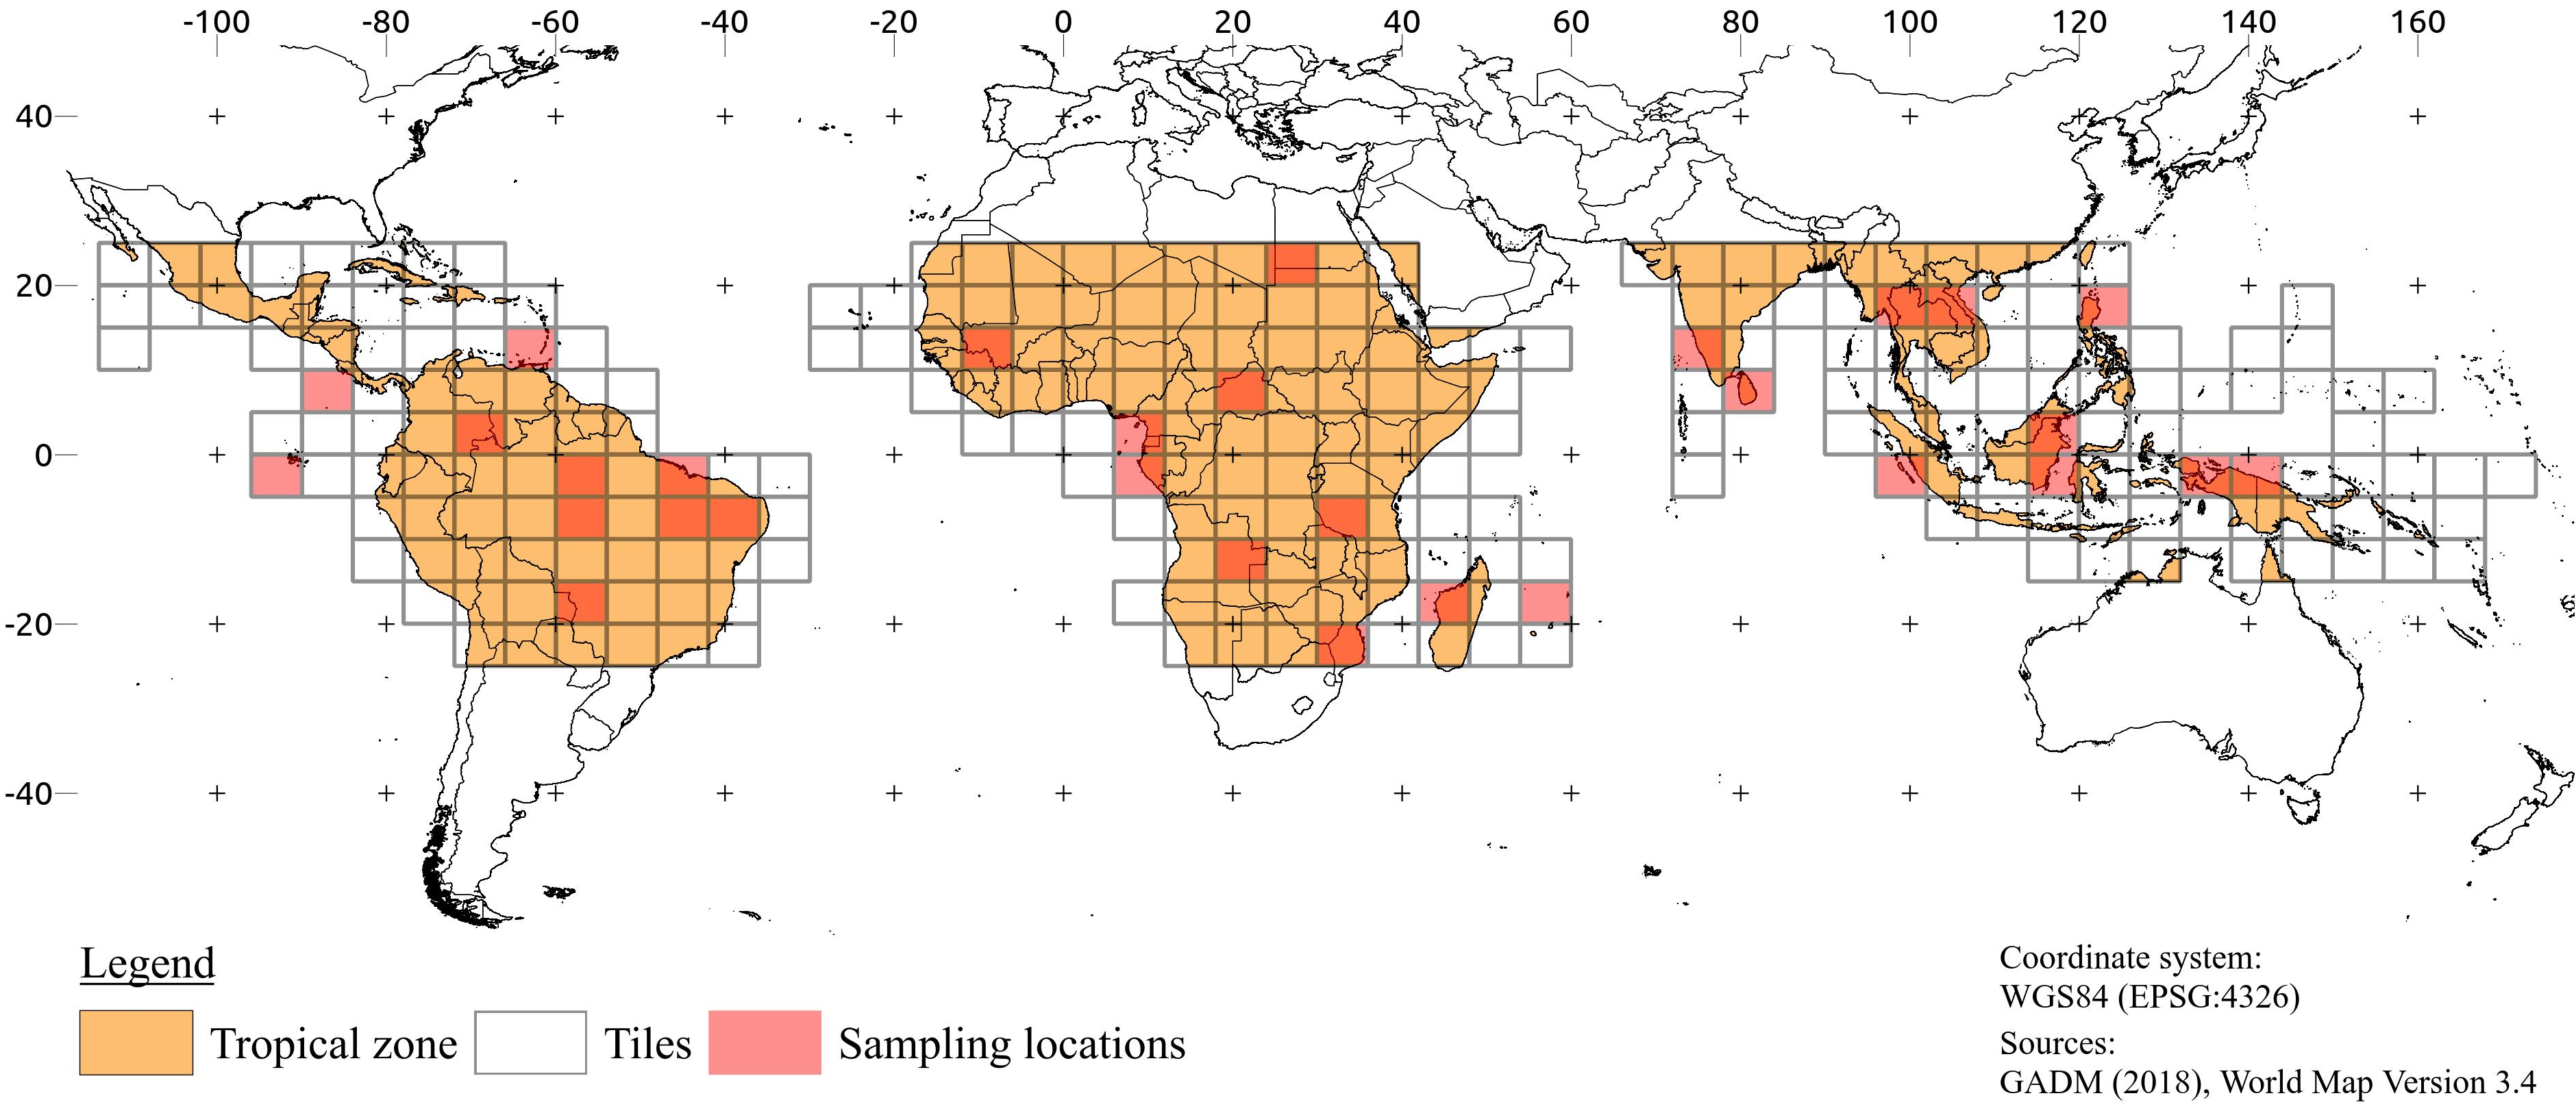
\includegraphics[scale=.97]{img/method_overview_frameless}
		\caption[Study extent]{Study extent and raster image tiles}
		\label{fig:studyextent}
	\end{figure}

	\subsubsection{Spatial data}
		\paragraph{Global Forest Change}
		\paragraph{GlobeLand30}
		\paragraph{Intact Forest Landscapes}
		\paragraph{Aboveground Woody Biomass}
		\paragraph{Global Soil Organic Carbon}
		\paragraph{Auxiliary}

	\subsubsection{Empirical data}
		\paragraph{Soil Organic Carbon}
		\paragraph{Ecosystem Service Values}


\subsection{Methods}
\label{subsec:methods}
%TODO need more speacking section headings
%TODO flowchart

	\subsubsection{Pre-processing}

	\subsubsection{Deforestation}
		\paragraph{Forest definition}
		\paragraph{Land use change driver}
		\paragraph{Accuracy assessment}

	\subsubsection{Emissions}
		\paragraph{Above ground biomass}
		\paragraph{Soil organic carbon change}

	\subsubsection{Ecosystem service values}
		\paragraph{Ecosystem service value loss}
		\paragraph{Ecosystem service value gain}

	\subsubsection{Binning analysis}
	%TODO x/y shift equations
		\begin{equation}
		\label{eq:paramters}
			R = \frac{\sqrt{2A}}{\sqrt[4]{27}} = \frac{D}{2} = \frac{d}{\sqrt{3}}
		\end{equation}
		\begin{equation}
		\label{eq:centerx}
			c_x = \frac{R\sqrt{3}}{2} 
		\end{equation}
		\begin{equation}
		\label{eq:centery}
			c_y = R
		\end{equation}
		\begin{equation}
		\label{eq:hexagon}
			\mathbf{H} =
			\begin{bmatrix}
				0 & c_x & 2c_x & 2c_x & c_x & 0 \\
				R\sin\left(\frac{7\pi}{6}\right) + c_y & 0 & R\sin\left(\frac{11\pi}{6}\right)+c_y & R\sin\left(\frac{\pi}{6}\right)+c_y & 2R & R\sin\left(\frac{5\pi}{6}\right)+c_y \\
				1 & 1 & 1 & 1 & 1 & 1
			\end{bmatrix}
		\end{equation}
		\begin{equation}
		\label{eq:translate}
		\mathbf{T} =
			\begin{bmatrix}
				1 & 0 & x_{off} \\
				0 & 1 & y_{off} \\
				0 & 0 & 1
			\end{bmatrix} \cdot \mathbf{H}
		\end{equation}
		\begin{equation}
		\label{eq:bounds}
			\mathbf{B} =
			\begin{bmatrix}
				x_1 & x_2 \\
				y_1 & y_2
			\end{bmatrix}
		\end{equation}
		\begin{equation}
		\label{eq:radius}
			R = \frac{\sqrt{2A}}{\sqrt[4]{27}}
		\end{equation}
		\begin{equation}
		\label{eq:percentage}
			y = \frac{P(y_2-y_1)}{100} + y_1
		\end{equation}
		\begin{equation}
		\label{eq:left}
			f^{-1}(y) =
			\begin{cases} 
				-\frac{y - y_1}{\tan{(\frac{\pi}{6}})} + \frac{x_1 + x_2}{2} & \text{if } y_1 \le y < y_1 + R\sin{(\frac{5\pi}{6})} \\
				x_1 & \text{if } y_1 + R\sin{(\frac{5\pi}{6})} \le y < R(\sin{(\frac{5\pi}{6})} + 1) \\
				\frac{y - y_2}{\tan{(\frac{\pi}{6}})} + \frac{x_1 + x_2}{2} & \text{if } R(\sin{(\frac{5\pi}{6})} + 1) \le y \le y_2
			\end{cases}
		\end{equation}
		\begin{equation}
		\label{eq:right}
			g^{-1}(y) = 
			\begin{cases} 
				\frac{y - y_1}{\tan{(\frac{\pi}{6}})} + \frac{x_1 + x_2}{2} & \text{if } y_1 \le y < y_1 + R\sin{(\frac{5\pi}{6})} \\
				x_2 & \text{if } y_1 + R\sin{(\frac{5\pi}{6})} \le y < R(\sin{(\frac{5\pi}{6})} + 1) \\
				-\frac{y - y_2}{\tan{(\frac{\pi}{6}})} + \frac{x_1 + x_2}{2} & \text{if } R(\sin{(\frac{5\pi}{6})} + 1) \le y \le y_2
			\end{cases}
		\end{equation}
		\begin{equation}
		\label{eq:line}
			\mathbf{L} =
			\begin{bmatrix}
				f^{-1}(y) & g^{-1}(y) \\
				y & y
			\end{bmatrix}
		\end{equation}
